%% Section: Using the debugger

Once the debugger's GUI loads, the programmer triggers the program execution by
clicking the \textit{Start} button. When starting by command line, the
application is automatically started. The program starts off displaying the user
and system entry points as a list of check boxes, freezing at the onset. The
user could choose to set breakpoints by clicking on the corresponding entry
points and kick off execution by clicking the \textit{Continue} Button. Figure
\ref{snapshot3} shows a snapshot of the debugger when a breakpoint is reached. 
The program freezes when a breakpoint is reached.

 
Clicking the \textit{Freeze} button during the execution of the program freezes
execution, while \textit{Continue} button resumes execution. \textit{Quit}
button can be used to abort execution at any point of time. Entities (for
instance, array elements) and their contents on any processor can be viewed at
any point in time during execution as illustrated in Figure \ref{arrayelement}.

\begin{figure}[]
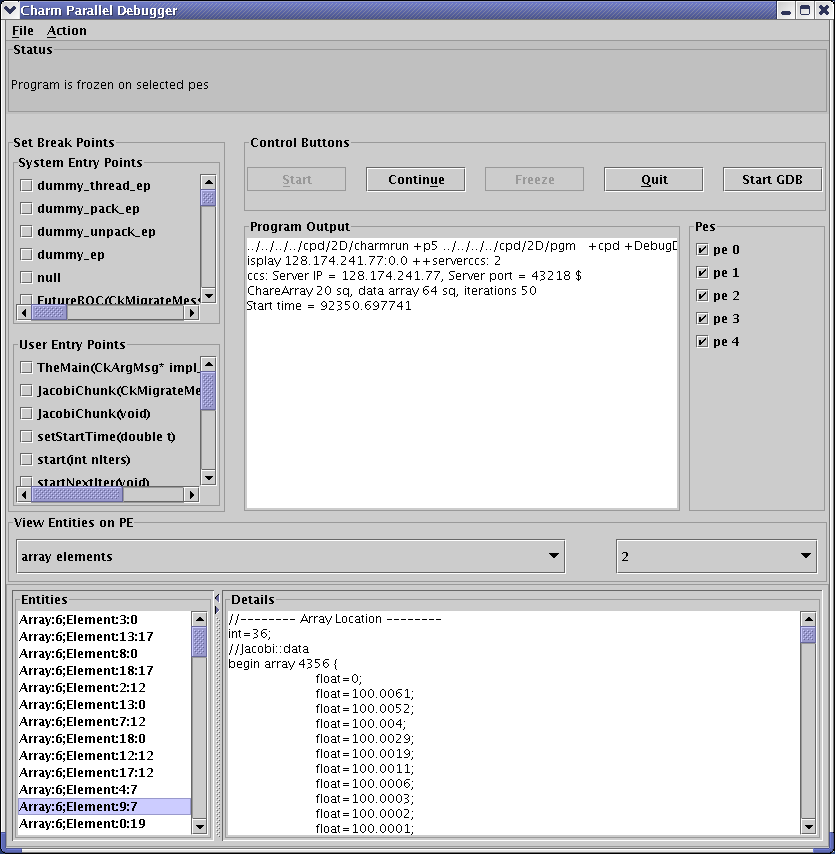
\includegraphics[scale=0.5, height=4in,width=3in]{figs/arrayelement}
\caption{Freezing program execution and viewing the contents of an array element using the Parallel Debugger}
\label{arrayelement}
\end{figure} 

Specific individual processes of the \charmpp{} program can be attached to instances of \textit{gdb} 
as shown in Figure \ref{gdb}. The programmer chooses which PEs to connect \textit{gdb} processes to via the checkboxes on the right side.
\emph{Note!} While the program is suspended in gdb for step debugging, the high-level features such as object inspection will not work.

\begin{figure}[ht!]
\centering
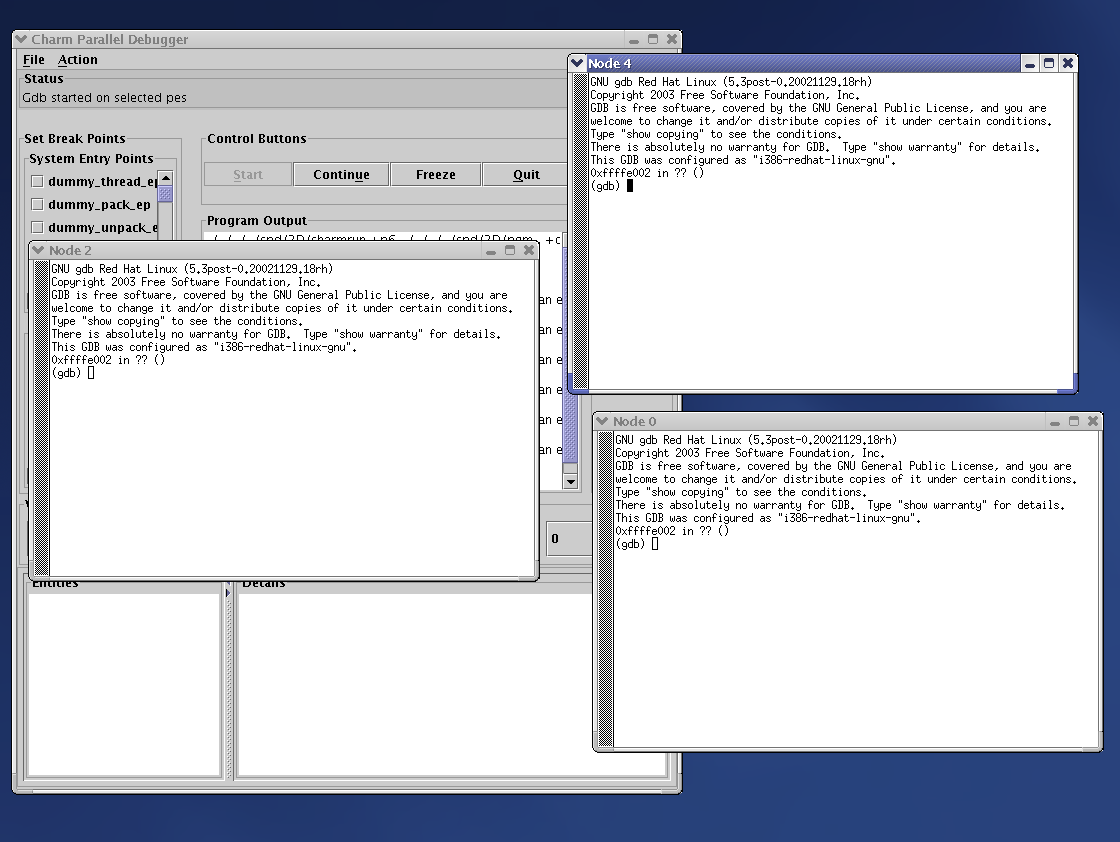
\includegraphics[width=6in]{figs/snapshot4-crop}
\caption{Parallel debugger showing instances of \textit{gdb}
open for the selected processor elements}
\label{gdb}
\end{figure}

\charmpp{} objects can be examined via  the \textit{View Entities on PE : Display} \ selector.  It allows the user to choose from  \textit{Charm Objects, Array Elements, Messages in Queue, Readonly Variables, Readonly Messages, Entry Points, Chare Types, Message Types and Mainchares}.  The right sideselector sets the PE upon which the request for display will be made. The user may then click on the \textit{Entity} to see the details. 

% The programmer can implement the function \texttt{pupCpdData(PUP::er
% \&)} for an array element and thereby control the information
% displayed by the debugger by choosing the data to be displayed and by
% inserting appropriate comments. An example is illustrated in Figure
% \ref{instr}.

% \begin{verbatim}
% // MyArray is a chare array where each array
% // element has a member variable data, 
% // which is an integer array

% void MyArray::pupCpdData(PUP::er &p) {
%   p.comment("contents of integer array: data");
%   p|data;  }
% \end{verbatim}

\subsubsection{Memory View}
\label{sec:memory}

The menu option Action~$\rightarrow$~Memory allows the user to display the
entire memory layout of a specific processor. An example is shown in
figure~\ref{fig:memory}. This layout is colored and the colors have the
following meaning:

\begin{figure}[ht!]
\centering
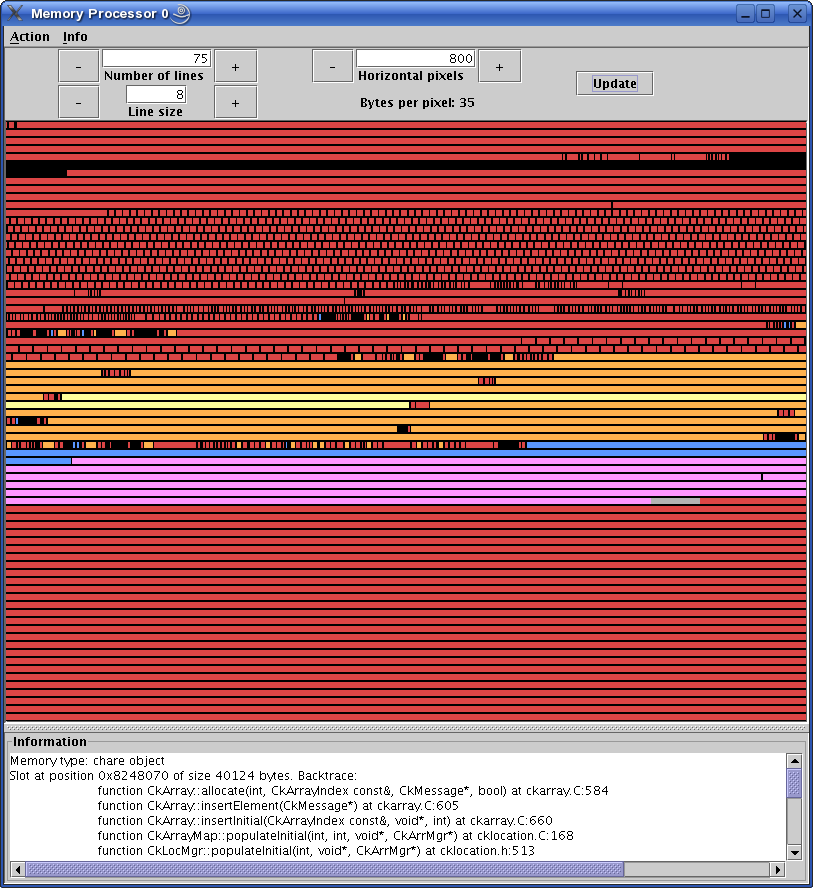
\includegraphics[scale=0.5]{figs/memoryView}
\caption{Main memory view}
\label{fig:memory}
\end{figure}

\begin{description}

\item[red] memory allocated by the \charmpp{} Runtime System;

\item[blue] memory allocated directly by the user in its code;

\item[pink] memory used by messages;

\item[orange] memory allocated to a chare element;

\item[black] memory not allocated;

\item[gray] a big jump in memory addresses due to the memory pooling system, it represent a large portion of virtual space not used between two different zones of used virtual space address;

\item[yellow] the currently selected memory slot;

\end{description}

Currently it is not possible to change this color association. The bottom part
of the view shows the stack trace at the moment when the highlighted (yellow)
memory slot was allocated. By left clicking on a particular slot, this slot is
fixed in highlight mode. This allows a more accurate inspection of its stack
trace when this is large and does not fit the window.

Info~$\rightarrow$Show~Statistics will display a small information box like the
one in Figure~\ref{fig:memory-stat}.

\begin{figure}[ht!]
\centering
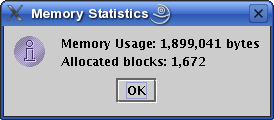
\includegraphics[scale=0.5]{figs/memoryStatistics}
\caption{Information box display memory statistics}
\label{fig:memory-stat}
\end{figure}

A useful tool of this view is the memory leak search. This is located in the
menu Action~$\rightarrow$~Search~Leaks. The processor under inspection runs a
reachability test on every memory slot allocated to find if there is a pointer
to it. If there is none, the slot is partially colored in green, to indicate its
status of leak. The user can the inspect further these slots. 
Figure~\ref{fig:memory-leak} shows some leaks being detected.

\begin{figure}[ht!]
\centering
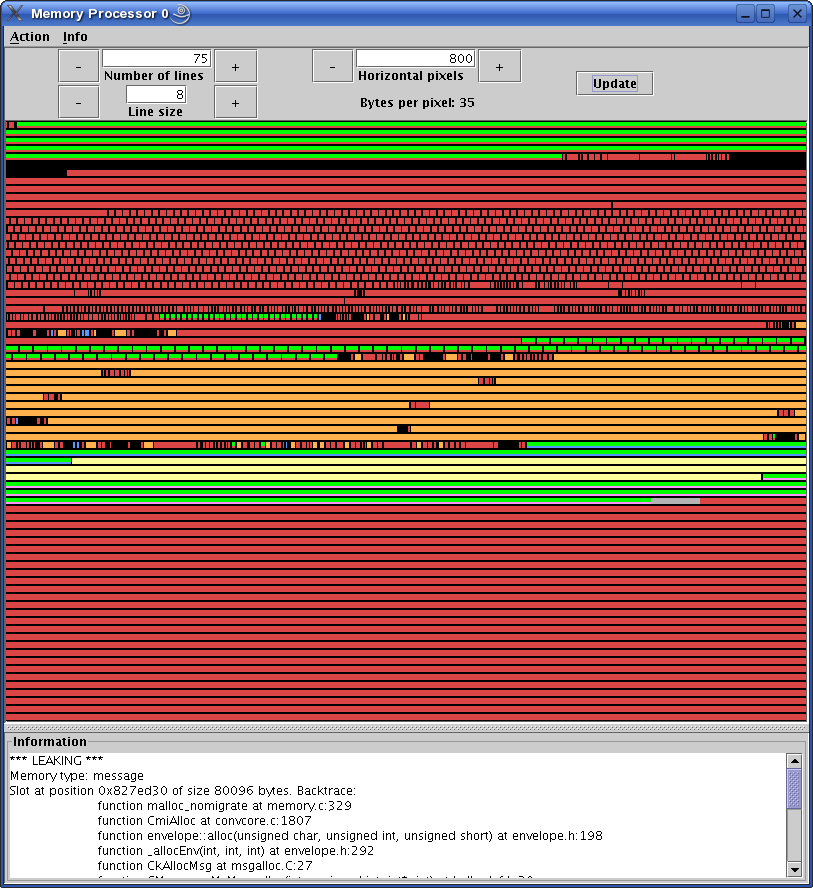
\includegraphics[scale=0.5]{figs/memoryLeaking}
\caption{Memory view after running the Search Leaks tool}
\label{fig:memory-leak}
\end{figure}

If the memory window is kept open while the application is unfrozen and makes
progress, the loaded image will become obsolete. To cope with this, the
``Update'' button will refresh the view to the current allocation status. All
the leaks that had been already found as such, will still be partially colored
in green, while the newly allocated slots will not, even if leaking. To update
the leak status, re-run the Search Leaks tool.

Finally, when a specific slot is highlighted, the menu
Action~$\rightarrow$~Inspect opens a new window displaying the content of the
memory in that slot, as interpreted by the debugger (see next subsection for
more details on this).

\subsubsection{Inspector framework}
\label{sec:inspector}

Without any code rewriting of the application, CharmDebug is capable of loading
a raw area of memory and parse it with a given type name. The result (as shown
in Fig.~\ref{fig:inspect}), is a browseable tree. The initial type of a memory
area is given by its virtual table pointer (\charmpp{} objects are virtual and
therefore loadbable). In the case of memory slots not containing classes with
virtual methods, no display will be possible.

\begin{figure}[ht!]
\centering
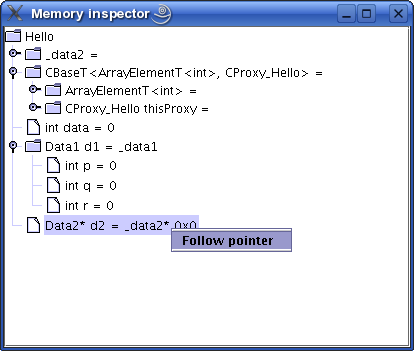
\includegraphics[scale=0.5]{figs/memoryInspector}
\caption{Raw memory parsed and displayed as a tree}
\label{fig:inspect}
\end{figure}

When the view is open and is displaying a type, by right clicking on a leaf
containing a pointer to another memory location, a popup menu will allow the
user to ask for its dereference (shown in Fig.~\ref{fig:inspect}). In this case,
CharmDebug will load this raw data as well and parse it with the given type name
of the pointer. This dereference will be inlined and the leaf will become an
internal node of the browse tree.

